% Created 2023-02-25 sam. 15:28
% Intended LaTeX compiler: pdflatex
\documentclass[11pt]{article}
\usepackage[utf8]{inputenc}
\usepackage[T1]{fontenc}
\usepackage{graphicx}
\usepackage{grffile}
\usepackage{longtable}
\usepackage{wrapfig}
\usepackage{rotating}
\usepackage[normalem]{ulem}
\usepackage{amsmath}
\usepackage{textcomp}
\usepackage{amssymb}
\usepackage{capt-of}
\usepackage{hyperref}
\author{Mattyas MARQUES}
\date{\today}
\title{Rapport groupe 142}
\hypersetup{
 pdfauthor={Mattyas MARQUES},
 pdftitle={Rapport groupe 142},
 pdfkeywords={},
 pdfsubject={},
 pdfcreator={Emacs 26.3 (Org mode 9.1.9)}, 
 pdflang={English}}
\begin{document}

\maketitle
\tableofcontents

\section{Problème}
\label{sec:org3295681}
\subsection{Modélisation des piece et du plateau}
\label{sec:org36ed440}
\subsubsection{Pieces<E>}
\label{sec:org88f7228}
\begin{enumerate}
\item Domino
\label{sec:org8ff8df6}
Cette classe est une extension de Piece<Integer> ce qui force l'utilisation des Integer pour les valeurs du tableau vals. L'Override de posable lui fait les vérifications nécessaires pour pouvoir poser sur le plateau. 
\item Carcassonne
\label{sec:org1a64977}
Cette Classe est une extension de Piece<ObjectCarcassonne> et gere elle meme la creation de pièces.
\item Généralisation des classes
\label{sec:org43697be}

Le but est de généraliser et forcer la création de toutes les fonctions dont le plateau pourrait avoir besoin ainsi il y a : 
\begin{enumerate}
\item Tout les champs
\begin{itemize}
\item Le tableau des valeur de E
\item La position relative de la piece par rapport au centre
\item Les pointeur vers les autres pieces dans les 4 direction
\item Des boolean indiquant pour chaque direction si il existe quelque chose
\end{itemize}
\item Certains getters
\item La fonctions \texttt{public void prepPlateau(List<Piece> posable)} qui va preparer le tableau pour le tour du joueur suivant
\item La fonction \texttt{tournerUnePiece()}
\item La fonction \texttt{contains(s(List<Piece> set ,int x , int y)}
\item La \texttt{equals(Piece obj)}
\item La fonction \texttt{abstract posable(String orientation , Piece pieceSurPlateau , Piece aPoser)}
\item La fonction \texttt{int comptePoint(Joueur j, Piece<E> up, Piece<E> right, Piece<E> down, Piece<E> left)}
\end{enumerate}
\end{enumerate}
\subsubsection{Plateau}
\label{sec:org5a2c425}
\begin{enumerate}
\item Les champs
\label{sec:org8b998f1}
Un premier champs qui est \texttt{Collection<Piece<E>> pieces} le but d'avoir une Collection est de ne pas avoir à chercher les doubles et pouvoir faire des action avec les stream de donnez et pouvoir créer des map pour l'affichage ou ne pas avoir de fixation au niveau de la taille ou longueur de notre modèle de donnée. Par exemple avec : \texttt{coll.stream().collect(Collectors.groupingBy(Piece::getY))} on peut facilement récupérer ligne à ligne le plateau sans avoir de cases vides comme dans un tableau. Et deux autres champs \texttt{public HashSet<Piece<E>> piecesLibre} et \texttt{public ArrayList<Piece<E>> piecesPosable} qui vont servir à garder en mémoire les pièces ou on peut poser un domino, et l'autre qui garde les endroits on ou pourra poser les pièces 
\item Les fonctions
\label{sec:orgf2bcc08}
\begin{enumerate}
\item \texttt{public HashSet<Piece<E>> freePiece()} qui va renvoyer un hashSet composer de toute les piece qui on au moins un coté libre
\item \texttt{public HashSet<Object[]> borderCombinaison(HashSet<Piece <E>> bordersE)} méthode qui elle renverra un HashSet avec tout les triplets ou on peut poser un domino et en plus l'index du côté sur lequel le triplet se trouve sur le domino 
\begin{itemize}
\item Le but d'utiliser ici des hashSet est de pouvoir ajouter les triplets sans ce soucier de double
\end{itemize}
\item \texttt{public int getMaxX()} et \texttt{public int getMaxY()} les deux méthodes elle renverront le minima et le maxima des positions en X des pièces du plateau courant
\item \texttt{public int getMaxY()} et \texttt{public int getMaxY()} les deux méthodes, elles renverront le minima et le maxima des positions en Y des pièces du plateau courant
\item \texttt{public boolean placePiece (Piece piece , int x , int y , Joueur j)} cette méthode va servir à verifier si la Piece piece est posable en x , y et la placera si c'est possible
\item \texttt{public void place(Piece piece , int x , int y , Joueur j)} méthode qui place la Piece piece
\item \texttt{public void prepPlateau()} prépare le plateau pour pouvoir monter et récupérer toutes les coordonnées ou sont posable des pièces à ce tour avec le plateau actuel
\item \texttt{public int getMaxX()} et \texttt{public int getMaxY()} les deux methodes, elles renverront le minima et le maxima des positions en X des pièces du plateau courant
\item \texttt{public int getMaxY()} et \texttt{public int getMaxY()} les deux methodes, elles renverront le minima et le maxima des positions en Y des pièces du plateau courant
\end{enumerate}
\end{enumerate}

\subsubsection{Joueur}
\label{sec:org3a97a68}
\begin{enumerate}
\item \texttt{whatToDo(Controleur c)} qui va demander au controleur de lui renvoyer l'action du joueur
\item \texttt{draw(Plateau plateau , Jeu jeu)} va piocher et en fonction du plateau actuel piochera un piece avec de grande chance d'etre posable
\item \texttt{playerAction(Controleur controleur , Plateau plateau)}
\item \texttt{dumpCurrent()} Défausse la pièce pioché en mettant la valeur de la pièce à null.
\item \texttt{addPoints(int comptePoint)} ajoute les points au joueur
\end{enumerate}
\begin{enumerate}
\item Bot normal
\label{sec:org1c36f65}
\begin{enumerate}
\item \texttt{public boolean playerAction(Controleur c,Plateau p)} Reprend la fonction prise dans les fonctions gérant les tours, on créer un tableau tabPosable bidimensionnel de int, on teste chaque pièce libre du plateau pour tester si la pièce piochée rentre dans une case, si elle n'y rentre pas -1 est placé dans le tableau. On test ensuite si le tableau est rempli de -1 si oui il défausse la carte, si non il choisit une pièce au hasard et pose donc la pièce.
\item \texttt{private void tournePiece(int i)} sert à tourner la piece i fois.
\item \texttt{private static boolean isEmpty(int[][] tab)} sert à regarder si le tableau est remplis de -1.
\end{enumerate}
\end{enumerate}
\subsubsection{Jeu}
\label{sec:orgc92782c}
\begin{enumerate}
\item \texttt{public boolean tour()} permet de gérer automatiquement un tour et envoi un boolean true si c'est la fin d'une partie.
\item \texttt{public void play(boolean isDomino)} lance la parti et fait notamment un while(!tour)\{\} qui permet de jouer tour apres tour.
\item \texttt{private void win()} Affiche le classement des joueurs en appelant la fonction \texttt{afficheClassement()} de la class Controleur.
\item \texttt{public int getJoueursPoints(int indJoueur)}  Getter qui renvois le nombre de point du joueur, l'argument est l'indice du joueur permettant de retrouver simplement le joueur.
\item \texttt{public String getJoueursName(int indJoueur)} Getter qui renvois le nom du joueur, l'argument est l'indice du joueur permettant de retrouver simplement le joueur.
\item \texttt{public void nextPlayer()} augmente de 1 l'indice et le remets au premier indice s'il est nécessaire
\item \texttt{public Object[][] getWinners()} Renvois le classement des joueurs sous forme de tableau.
\end{enumerate}
\subsection{Généricité et intelligence des placement des fonctions}
\label{sec:org7931746}
Cette partie nous a causé beaucoup de problèmes en effet la différence entre une Piece et une Piece<?> nous a été difficile à comprendre et interpréter. Cette notion nous a causé tant de problèmes que le fait de pouvoir poser des pions n’a pas été réalisé à cause de cette utilisation de la généricité et de la mauvaise gestion que nous en avons eu. 
\subsection{Générer des pieces jouables}
\label{sec:orgad9d938}
Pendant un long moment au début du projet ce problème nous a fait réfléchir. Comment rendre le jeu jouable, nous avons décidé de trouver un moyen de toujours récupérer des triplets de chiffres posables. En faisant le tour du terrain nous récupérons tous les triplets ou on peut poser une pièce et on en choisit entre 0 et 4 au hasard pour en faire une nouvelle pièce au detail près que nous ne mettons pas le triplet comme ça dans la nouvelle pièce nous inversons ce triplet pour que le domino soit effectivement posable. 
\section{Representation graphique des classes}
\label{sec:orgee4c2f8}
\begin{center}
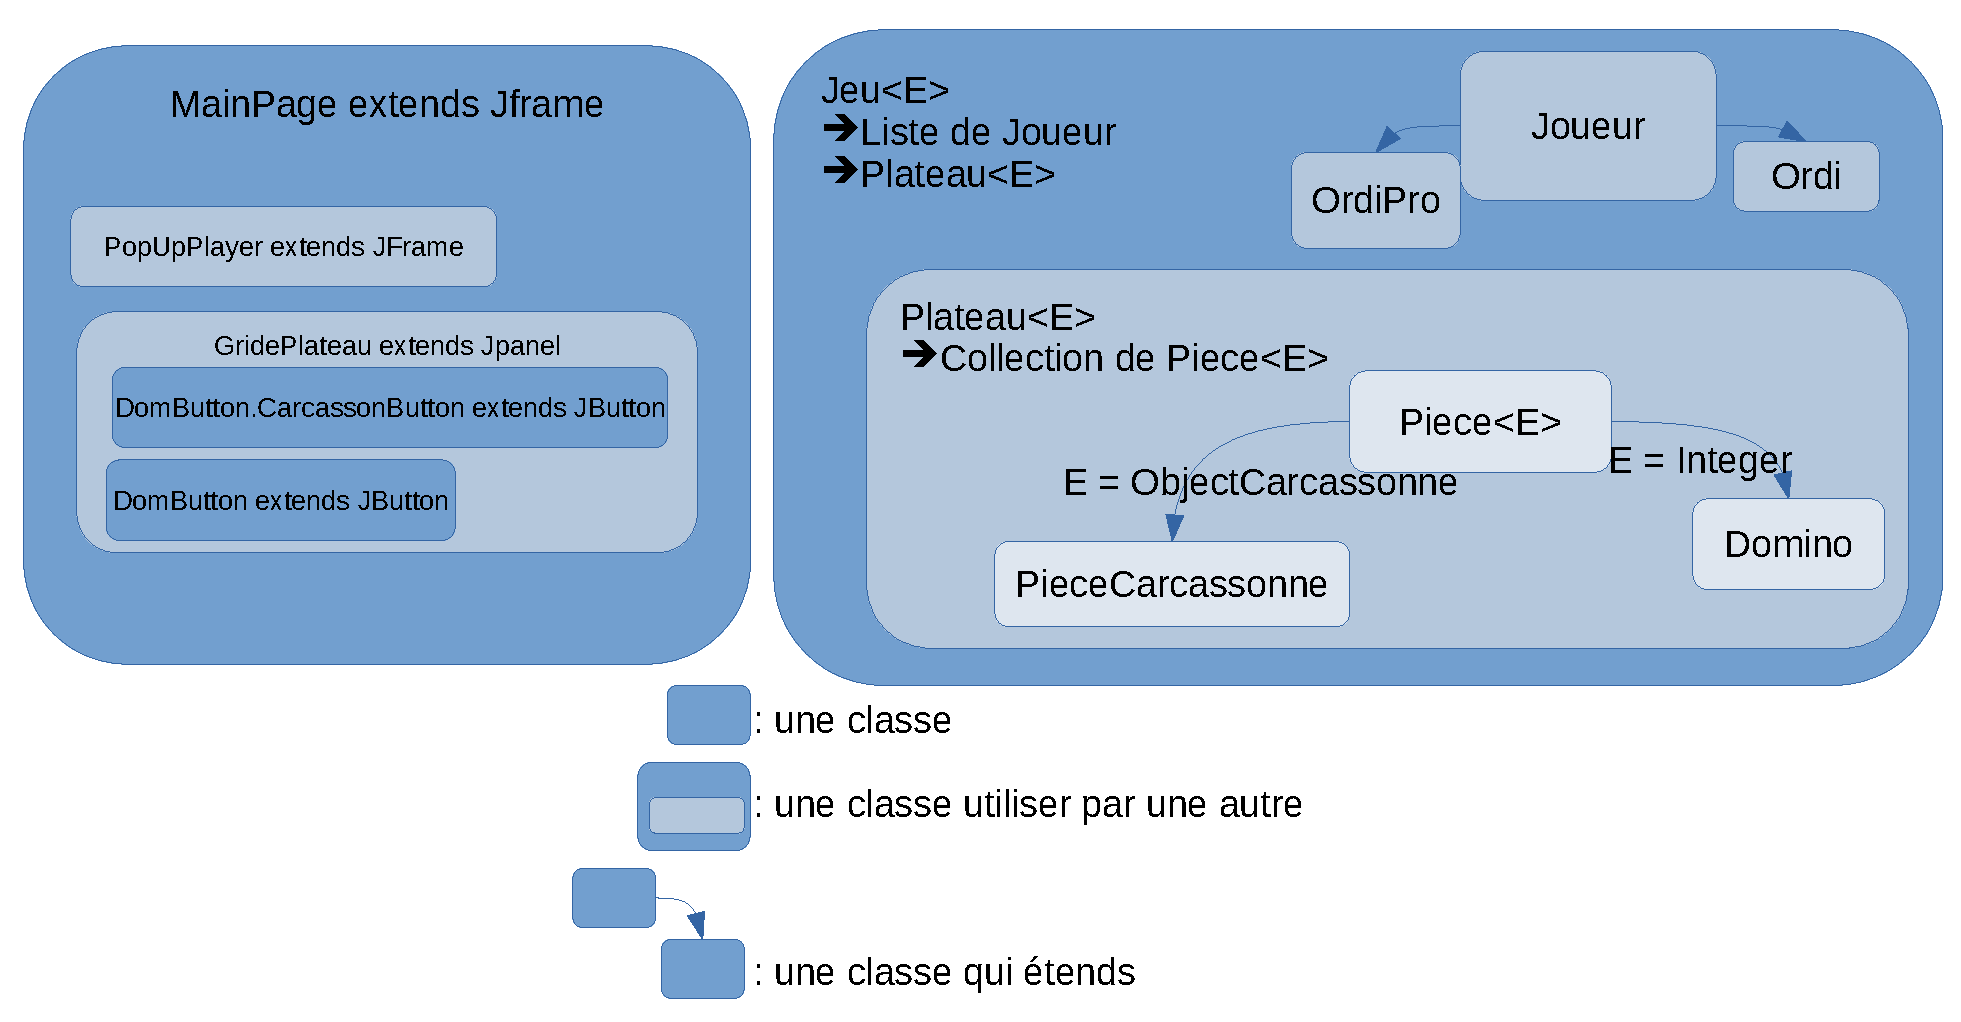
\includegraphics[width=.9\linewidth]{./SchemaClasses.pdf}
\end{center}
\section{Partie du cahier des charges traité}
\label{sec:orgdc2e19e}
\subsection{Interface Textuels}
\label{sec:org1bb8284}
Chaque fonction servira à imprimer dans le terminal ou déclarer l'interface graphique. Chaque fonction est nommée après ce qu’elle fait toutes les fonctions askQuelQueChose() seront des fonctions que le contrôleur récupère pour interpréter les données et les transmettre au model. Au contraire chaque fonction afficheQuelqueChose() est utilisée dans le sens inverse et affichera les données traitées par le contrôleur récupéré de l'état actuel du model. 
\begin{enumerate}
\item \texttt{public <E> void afficheListePiece(Collection<Piece<E>> list)}
\item \texttt{public <E> void afficheListePiecePosable(Collection<Piece<E>> list , ArrayList<Piece<E>> listeWherePosable)}
\item \texttt{private <E> void afficheListePieceLine(Collection<Piece<E>> coll , int line)}
\item \texttt{private <E> void afficheListePieceLinePos(Collection<Piece<E>> coll , int line , List<Piece<E>> listeWherePosable)}
\item \texttt{public void afficheMain (Piece p)}
\item \texttt{public void affichePiece(Piece p)}
\item \texttt{private String posableInd(int i)}
\item \texttt{public void affichePointJoueurs(String playerName , int joueursPoints)}
\item \texttt{public String askWhereToPlay(String name)}
\item \texttt{public String askWhereWhatToDo()}
\item \texttt{public void afficheClassement(ArrayList<Joueur> joueurs)}
\item \texttt{public String askToTurn()} Demande si le joueur veut tourner la pièce.
\item \texttt{public String askToDump()} Demande si le joueur veut défausser la pièce et passer son tour.
\item \texttt{public String askPlayers()} Demande le nombre de Joueur présent dans la partie.
\item \texttt{public String askBots()} Demande le nombre de Bots présent dans la partie.
\item \texttt{public String askName(int i)} Demande le nom du joueur à l'id i.
\item \texttt{public String askTuiles()} Demande le nombre de tuiles présent dans la partie.
\item \texttt{public void afficheActualPlayer(String name, int points)} Affiche le nombre de points du joueur.
\end{enumerate}
\subsection{Règles du jeu de domino}
\label{sec:org2c6f352}
Toutes les règles sont présentes dans les deux versions du jeux, nous pouvons poser tourner une pièce gagner des points, passer notre tour, abandonner et gagner.
\subsection{Règles de Carcassonne}
\label{sec:orgc73cb78}
Les règles de Carcassonne nous ont posé un problème au niveau du code avec le placement d'un pion à cause de la généricité de notre code et la manière dont on a construit et géré cela. Mais le placement d'une pièce est possible.
\subsection{Interface graphique}
\label{sec:orgd2768ac}
Cette interface graphique ce sépare en 4 classes et deux JFrames
\subsubsection{JFrame des Joueurs}
\label{sec:org2acc656}
Ce JFrame est la pour montrer la pièce courante du joueur, il est composé de 4 boutons qui sont : Piocher ; Pivoter ; Abandonner/Give Up ; et Passer. Chaque bouton porte le nom de son action 
\subsubsection{JFrame MainPage}
\label{sec:org6c53f87}
Cette JFrame est là pour accueillir le plateau et les menus.
\begin{enumerate}
\item Le plateau
\label{sec:org9a81476}
Le plateau est assuré par la classe GridPlateau qui affichera tous les dominos/tuiles présentes sous forme de boutons et plus précisément d'un objet créer par nous qui étend le JButton. 
\item Les Menus
\label{sec:org8297c7f}
Le premier menu est simple et sous la forme de deux boutons propose de choisir les dominos ou Carcassonne. Dans les deux cas appuyer sur un bouton mènera vers un menu qui pour les dominos propose de configurer le nombre de joueurs, le nombre de bots set le nombre de dominos qu'on veut utiliser. Pour Carcassonne les mêmes choix sont proposés a la différence que le nombre de tuiles est fixé et inchangeable.
\end{enumerate}
\subsection{HAL 9000}
\label{sec:org3b46aa2}
\begin{enumerate}
\item \texttt{public boolean playerAction(Controleur c,Plateau p)} Reprend la fonction prise dans les fonctions gérant les tours, on créer un tableau tabPosable bidimensionnel de int, on test chaque piece libre du plateau pour tester si la piece piochée rentre dans une case et rentre le nombre de point de celle ci, si elle n'y rentre pas -1 est placé dans le tableau. On test ensuite si le tableau est remplis de -1 si oui il défausse la carte, si non il choisit la piece qui lui rapporte le plus de point et la pose ensuite.
\item \texttt{private void tournePiece(int i)} sert à tourner la piece i fois.
\item \texttt{private static boolean isEmpty(int[][] tab)} sert à regarder si le tableau est remplis de -1.
\item \texttt{private static int max2(int[][] tab)} sert à renvoyer l'indice i ou se trouve la piece qui rapporte le plus de point.
\item \texttt{private static int max(int[] tab)} sert à renvoyer l'indice j ou se trouve la piece qui rapporte le plus de point.
\end{enumerate}
\end{document}
